\subsection{Problem}

\renewcommand{\theequation}{\theenumi}
\begin{enumerate}[label=\thesection.\arabic*.,ref=\thesection.\theenumi]
\numberwithin{equation}{enumi}
	\item Without using distance formula, show that the points
	\begin{multline}
	\vec{A} = \myvec{-2\\-1} \quad \vec{B} = \myvec{4\\0} \quad \vec{C} = \myvec{3\\3}\text{ and }\vec{D} = \myvec{-3\\2} 
	\end{multline}
	are the vertices of a parallelogram.
The following python code computes the area of $\triangle$ABC in Fig.\ref{fig:qfour}.
	\begin{lstlisting}
	./codes/quadrilateral/q4.py
	\end{lstlisting}
	
	\solution As the direction vectors,
	\begin{align}
	\vec{A - B}=\vec{D - C}
	\\
	\vec{A - D}=\vec{B - C}
	\end{align}
	
	\begin{figure}[!ht]
	\centering
	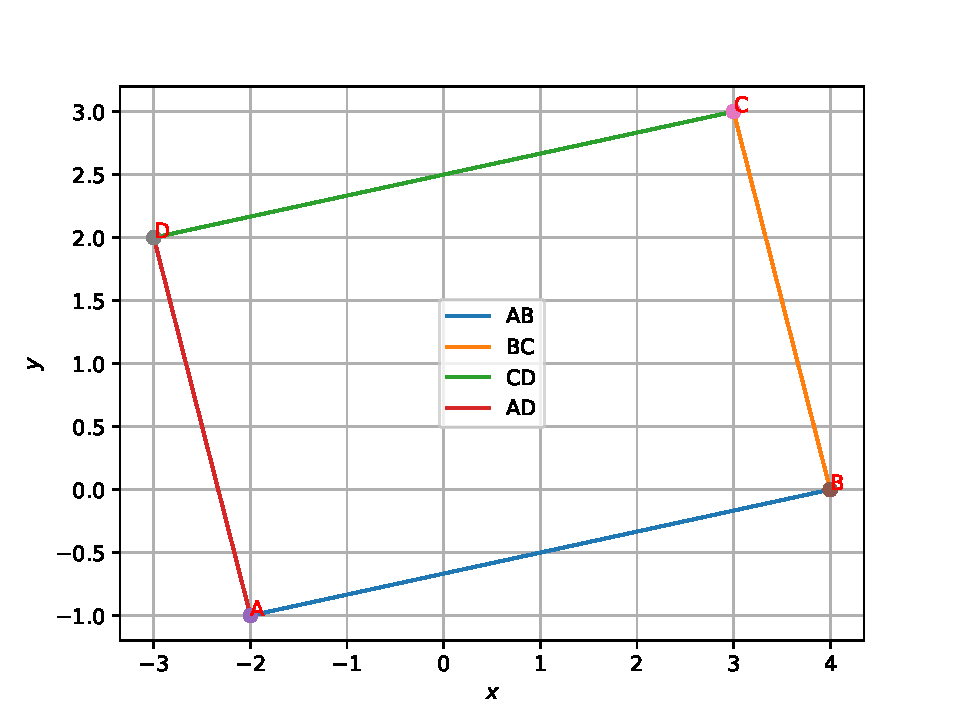
\includegraphics[width=\columnwidth]{./figs/quadrilateral/q4.pdf}
	\caption{Parallelogram of Q.2.2.5}
	\label{fig:qfour}	
	\end{figure}
	
	\begin{multline}
	\implies \vec{AB} \parallel \vec{CD}\text{ and }\vec{AD} \parallel \vec{BC}
	\\
	\therefore \vec{ABCD}\text{ is a parallelogram.}
	\end{multline}
\end{enumerate}
